%% 
%% Copyright 2007, 2008, 2009 Elsevier Ltd
%% 
%% This file is part of the 'Elsarticle Bundle'.
%% ---------------------------------------------
%% 
%% It may be distributed under the conditions of the LaTeX Project Public
%% License, either version 1.2 of this license or (at your option) any
%% later version.  The latest version of this license is in
%%    http://www.latex-project.org/lppl.txt
%% and version 1.2 or later is part of all distributions of LaTeX
%% version 1999/12/01 or later.
%% 
%% The list of all files belonging to the 'Elsarticle Bundle' is
%% given in the file `manifest.txt'.
%% 

%% Template article for Elsevier's document class `elsarticle'
%% with numbered style bibliographic references
%% SP 2008/03/01

\documentclass[preprint,12pt, a4paper]{elsarticle}

%% Use the option review to obtain double line spacing
%% \documentclass[authoryear,preprint,review,12pt]{elsarticle}

%% For including figures, graphicx.sty has been loaded in
%% elsarticle.cls. If you prefer to use the old commands
%% please give \usepackage{epsfig}

%% The amssymb package provides various useful mathematical symbols
\usepackage{minted}
\usepackage{amssymb}
\usepackage{hyperref}
\usepackage{xcolor}
\usepackage{todonotes}

\usepackage{rotating}
\setlength{\parindent}{0pt}
%% The amsthm package provides extended theorem environments
%% \usepackage{amsthm}

%% The lineno packages adds line numbers. Start line numbering with
%% \begin{linenumbers}, end it with \end{linenumbers}. Or switch it on
%% for the whole article with \linenumbers.
%\usepackage{lineno}

\journal{SoftwareX}

\begin{document}
\renewcommand{\labelenumii}{\arabic{enumi}.\arabic{enumii}}

\begin{frontmatter}
%--- INSTRUCTIONS TO BE DELETED OR COMMENTED BEFORE SUBMISSION 

% {\large\textbf{SoftwareX article template Version 4 (November 2023)}}
%   Before you complete this template, a few important points to note:
%   \begin{itemize}
% \item	This template is for an original SoftwareX article. If you are submitting an update to a software article that has already been published, please use the Software Update Template found on the Guide for Authors page.
% \item	The format of a software article is very different to a traditional research article. To help you write yours, we have created this template. We will only consider software articles submitted using this template.
% \item	It is mandatory to publicly share the code/software referred to in your software article. You’ll find information on our software sharing criteria in the SoftwareX \href{https://www.elsevier.com/journals/softwarex/2352-7110/guide-for-authors}{Guide for Authors}.  
% \item	It’s important to consult the \href{https://www.elsevier.com/journals/softwarex/2352-7110/guide-for-authors}{Guide for Authors} when preparing your manuscript; it highlights mandatory requirements and is packed with useful advice.
% \end{itemize}

\title{ObServML: Deployable Python application for compact and modular systems monitoring}

%% use optional labels to link authors explicitly to addresses:
%% \author[label1,label2]{}
%% \address[label1]{}
%% \address[label2]{}

\author[1]{Ádám Ipkovich}
\author[1]{János Abonyi}
\author[1]{Alex Kummer}
\address[1]{\orgdiv{HUN-REN-PE Complex Systems Monitoring Research Group}, \orgname{University of Pannonia}, \orgaddress{\city{Veszprém}, \postcode{H-8200},  \country{Hungary}}}

\begin{abstract}
ObservML enables the combination of training and deploying ML monitoring models within a single microservices-based system. Its application focuses on monitoring problems that can be solved with fault detection and isolation (FDI), time series analysis, and process mining through an operator-friendly and adaptable framework based on MLOps practices. The framework is developed to connect to RabbitMQ for real-time data communication and MLflow for model versioning. It supports a wide range of machine learning techniques, including decision trees, autoencoders, and time series models, providing a robust toolkit for anomaly detection and predictive maintenance, and can be extended as required. 
\end{abstract}
% \textit{Ca. 100 words. The abstract is followed by a maximum of six keywords
% and some mandatory and optional metadata.}
% \textit{Your main body of text (sections 1-5 below) should be a maximum 6 pages in total (excluding metadata, tables, figures, references) with a 3000-word limit (we ask that more priority is placed on the word limit versus the page count). Though we strictly insist on the author following the template, in exceptional circumstances, we can be flexible with the page numbers and word limit. In such cases, it should be discussed with the managing editor or publisher prior to submission. All queries regarding the same can be reached at softwarex@elsevier.com.}


\begin{keyword}
MLOps \sep monitoring \sep Machine learning \sep Deep learning \sep Fault detection
\end{keyword}
%% PACS codes here, in the form: \PACS code \sep code

%% MSC codes here, in the form: \MSC code \sep code
%% or \MSC[2008] code \sep code (2000 is the default)



\end{frontmatter}

%\linenumbers

\section*{Metadata}
\label{metadata}
\begin{table}[!h]
\begin{tabular}{|l|p{6.5cm}|p{6.5cm}|}
\hline
\textbf{Nr.} & \textbf{Code metadata description} & \textbf{Metadata} \\
\hline
C1 & Current code version & v1.0.0 \\
\hline
C2 & Permanent link to code/repository used for this code version & \textcolor{red}{SoftwareX}  \\
\hline
C3  & Permanent link to Reproducible Capsule & \url{https://hub.docker.com/repository/docker/ipkovichadam/observml/general}\\
\hline
C4 & Legal Code License   & MIT \\
\hline
C5 & Code versioning system used & git \\
\hline
C6 & Software code languages, tools, and services used &  Python, Docker, RabbitMQ, Mlflow, FastAPI, Streamlit   \\
\hline
C7 & Compilation requirements, operating environments \& dependencies & Provided in requirements.txt / pyproject.toml \\
\hline
C8 & If available Link to developer documentation/manual & \url{https://adamipkovich.github.io/observml/} \\
\hline
C9 & Support email for questions &  ipkovichadam@gmail.com\\
\hline
\end{tabular}
\caption{Code metadata (mandatory)}
\label{codeMetadata} 
\end{table}


\begin{table}[!h]
\begin{tabular}{|l|p{6.5cm}|p{6.5cm}|}
\hline
\textbf{Nr.} & \textbf{(Executable) software metadata description} & \textbf{Please fill in this column} \\
\hline
S1 & Current software version & 1.0.0 \\
\hline
S2 & Permanent link to executables of this version  & \url{https://github.com/adamipkovich/observml.git} \\
\hline
S3  & Permanent link to Reproducible Capsule & \url{https://hub.docker.com/repository/docker/ipkovichadam/observml/general} \\
\hline
S4 & Legal Software License & MIT \\
\hline
S5 & Computing platforms/Operating Systems & Containerized \\
\hline
S6 & Installation requirements & Docker, for local development, python dependencies are provided in the pyproject.toml  \\
\hline
S7 & If available, link to user manual - if formally published include a reference to the publication in the reference list &  \url{https://adamipkovich.github.io/observml/} \\
\hline
S8 & Support email for questions & ipkovichadam@gmail.com\\
\hline
\end{tabular}
\caption{Software metadata (optional)}
\label{executabelMetadata} 
\end{table}


\clearpage

% \todo[inline]{LE KELL CSÖKKENTENI A SZÓSZÁMOT, MAX 3/6 oldal ábrák nélkül!!}

% \color{red}
% -> Intro 3-4 bekezdés
% -> Architektúra minimális, abstrakt elmagyarázása + eszközök megnevezése
% \color{black}

\section{Motivation and significance}
% \todo[inline]{Amit mi monitorozunk azér sok mindenre jó... általános rendszer ... during production helyett általánosabb...}


The detection of critical errors is of the utmost importance. Without a proper monitoring tool, it is increasingly difficult to find inefficiencies and errors in the system. Our goal is to establish an efficient, real-time monitoring platform that monitors real-time streamed data from multiple sources.

The contribution of fault detection and isolation (FDI) tools in modern industrial systems is critical to ensure state-of-the-art reliability, safety, and operational efficiency, so the industry increasingly relies on data-driven approaches. The demand for adjustable, efficient, and user-friendly tools to handle complex monitoring tasks has increased significantly \cite{ZONTA2020106889}. There are several monitoring tools, \textit{e.g.} advanced fault diagnosis analysis library in MatLab for large-scale models that have a Python implementation \citep{FRISK20173287}. The BibMon package for example provides several implemented monitoring tools \citep{MELO2024100182}, however, provides no deployment and MLOps features. Some solutions target very specific problems, such as digital twins to simulate sensors \citep{dig_twin}, system analysis to understand model behavior \citep{Schummer_Hyba_2022}. While there are innovative solutions to existing problems, such as monitoring earthquakes whose models can be adjusted \citep{LI2024105686}.

As opposed to Kubernetes-based orchestrators, such as Flyte and Kubeflow, our project focus on smaller applications. It is not computationally and cost efficient to use Kubernetes on such a scale. It also requires proper Kubernetes Operators to properly monitor the containers that could drive up the costs. Modern solutions end-to-end ML solution, such as Dataiku, often focus on cloud deployment, which could increase the costs significantly for developers/researchers who are not able to afford their own private cloud systems. Thus, we aim to provide a self-deployable pre-defined system for monitoring, while its modularity can reduce costs and improve the flexibility of ML model use.


We adhere to MLOps principles as predictive systems can provide more harm that benefit without proper specifications. As such, we define the following requirements to assure quality workflow in our package:
\begin{itemize}
\item Loosely coupled Architecture (Modularity) -- A flexible, microservices-based architecture.
\item Reproducibility -- Versioning, tracking and storing ML models
\item Orchestrated -- Configuration files to build and deploy ML models with
\item Continuous Testing -- Implement custom metrics, and KPIs
\item Continuous Delivery -- A system that is capable of exposing/deploying custom predictive functionalities
\item Continuous Training -- Retraining capabilities affected by real-time data
\item Continuous Monitoring -- Performance monitoring of ML Models 
\end{itemize}


Motivated by this requirement specification, we developed a Python package for modular monitoring applications tailored to fault detection and isolation workflows. Our system is built on a microservices architecture leveraging Docker for containerization, RabbitMQ for efficient data handling, and MLflow \citep{mlflow} for experiment tracking. It supports diverse machine learning models, including decision trees, autoencoders, ARIMA, LSTM, \textit{etc}. The modularity of the package allows for straightforward model substitution and customization, enabling users to fine-tune configurations to suit specific industrial datasets and requirements. The models are trained based on one set of instructions (Hydra/YAML configuration files \citep{Yadan2019Hydra}) that the operators provide so that they do not have to manually provide code for specific setups. These features ensure that operators deploy models and monitor their systems in real-time. 


% Motivated by this gap, we developed a Python package for modular monitoring applications tailored to integrate fault detection and isolation workflows seamlessly. Our system is built on a microservices architecture leveraging Docker for containerization, RabbitMQ for efficient data handling, and MLflow \citep{mlflow} for experiment tracking. It supports diverse machine learning models, including decision trees, autoencoders, ARIMA, LSTM, \textit{etc}. The modularity of the package allows for straightforward model substitution and customization, enabling users to fine-tune configurations to suit specific industrial datasets and requirements. The models are trained based on one set of instructions (Hydra/YAML configuration files \citep{Yadan2019Hydra}) that the operators provide so that they do not have to manually provide code for specific setups. These features ensure that operators deploy models and monitor their systems in real-time. 

\clearpage
Figure \ref{concept_map} presents the main concepts of the package.
\begin{figure}[h]
\centering
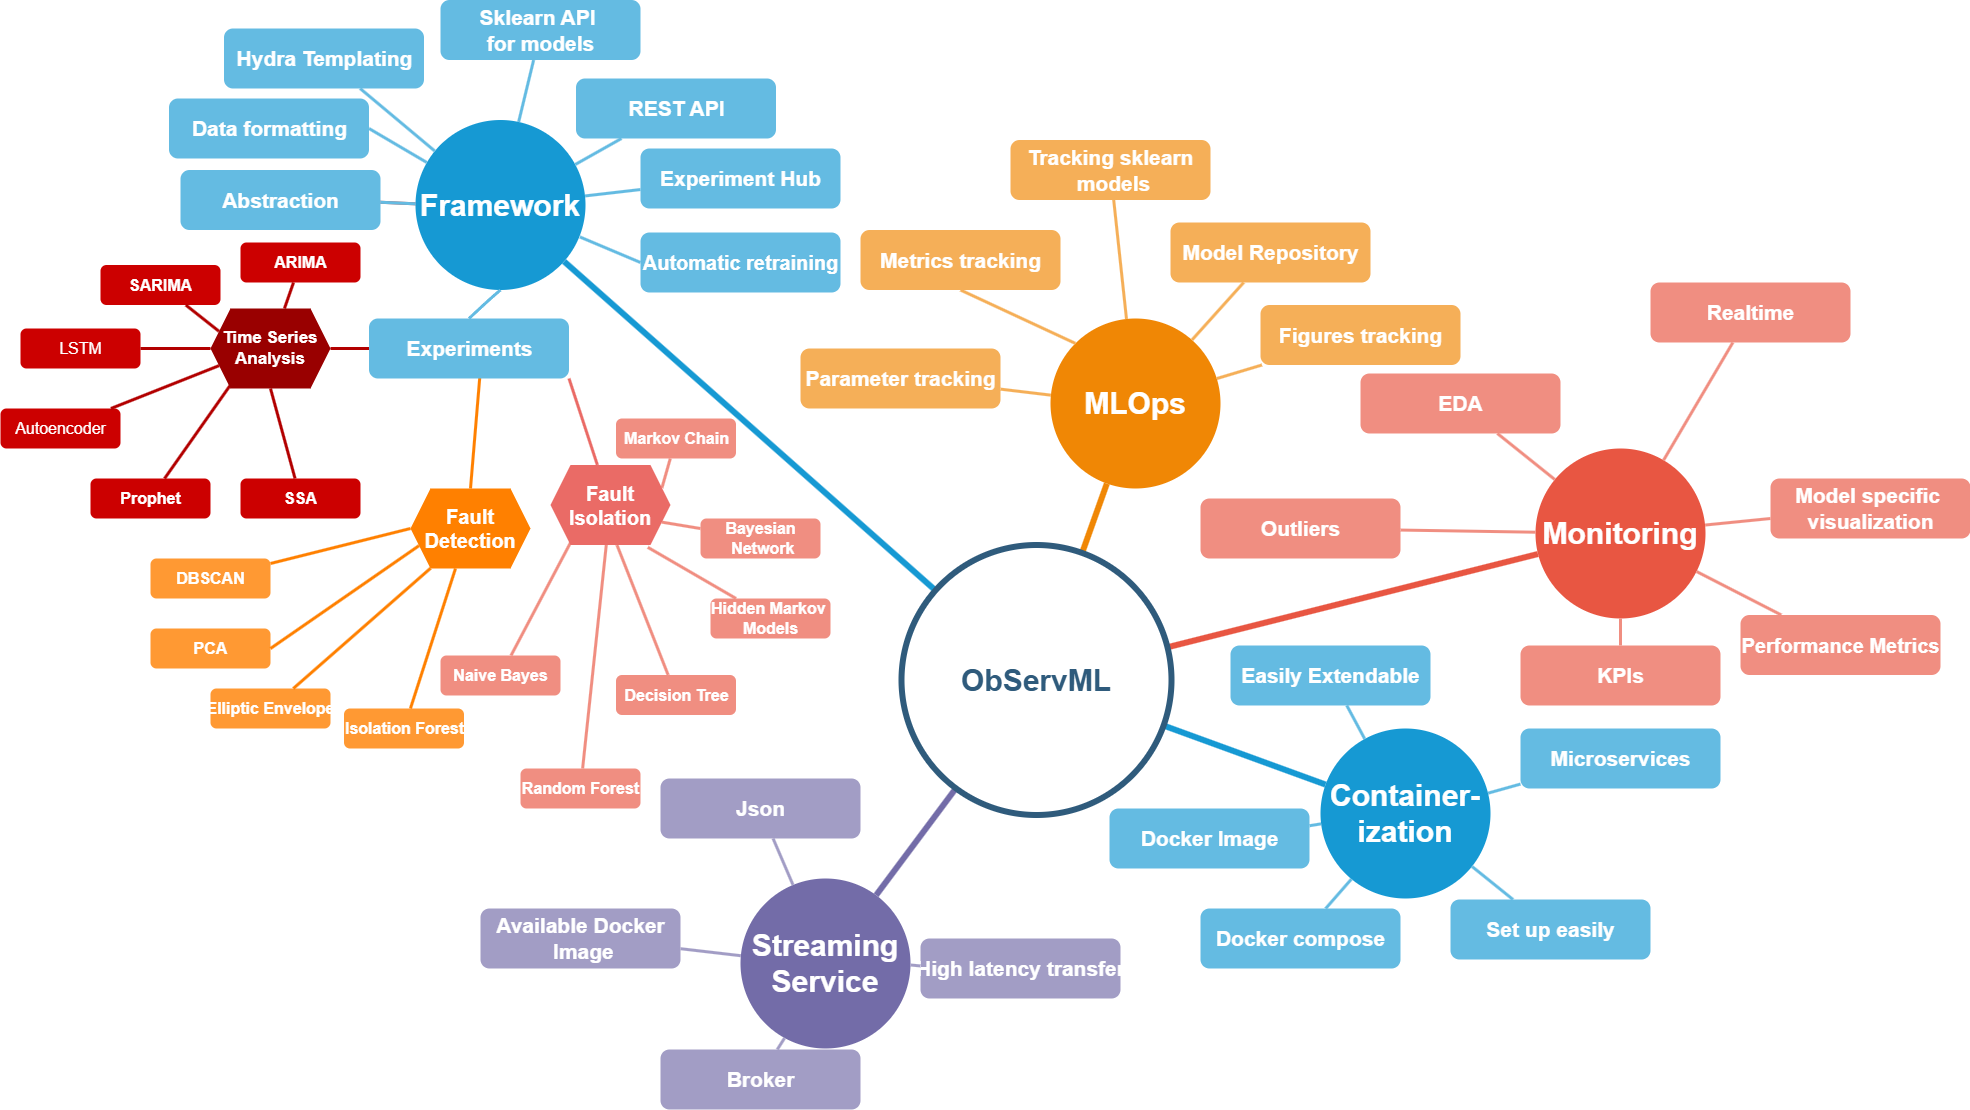
\includegraphics[width=0.9\textwidth, angle=90]{figs/concept_map.png}
\caption{Concept map of the developed CMMA python package. The colored circles denote the microservices, whilst rectangles present a feature of the service. For the Experiments features, more concrete information is depicted in forms of the problems it can solve (fault detection, fault isolation and time series analysis). Process mining is not on the concept map as it is only an experimental feature}
\label{concept_map}
\end{figure}

Adopting Internet of Things (IoT) technologies and Industry 4.0 practices can significantly enhance industrial performance \citep{BUCHI2020119790}. However, the presence of sensors does not inherently provide additional value; what really contributes to performance is the analysis of this data. A key focus in manufacturing remains cost reduction, which can be achieved through approaches such as operator behavior analysis \citep{GLADYSZ2023160}, manufacturing process optimization \citep{SOORI2023100017}, alarm management \citep{alarm_management}, and predictive maintenance \citep{ZONTA2020106889}.

Industry 4.0 faces several challenges, including handling anomalies and noisy data, addressing the lack of labeled datasets, and managing efficiency with large-scale data \citep{NUNES202353}. Proper infrastructure, such as RabbitMQ and cloud services, can address the challenges of big data. For typical data-driven predictive maintenance tasks, simpler models like Principal Component Analysis (PCA) can effectively tackle the problem of the lack of labeled data \citep{NUNES202353}.

To further reduce the strain on engineers, we have developed the ObServML package for predictive maintenance. This package includes infrastructure for real-time monitoring with fault detection approaches, fault isolation for understanding machine states, time-series analysis to forecast sensor values and detect deviations from expected outcomes. We also provide some options for process mining to analyze machine and operator logs. 


The paper presents the architecture, framework, and use of the package for predictive maintenance. By combining modularity with an operator-friendly design, the system aims to provide a straightforward predictive maintenance application. We demonstrate its utility through fault detection and isolation, showcasing its ability to transform monitoring and operational efficiency in an industrial environment. The contribution of the package is as follows:
\begin{itemize}
\item A flexible, microservices-based architecture leveraging Docker (Compose), RabbitMQ, and MLflow for containerization, data handling, and model tracking.
\item A modular system enabling seamless configuration and substitution of machine learning models from a wide range of packages for diverse datasets and tasks so that operators do not have to write code themselves.
\item Easily extendable framework for both experiments and models.
\item Ease of integration with data collectors and databases through REST API-based deployment of the models.
\item Adherence to MLOps principles, ensuring scalability, reproducibility, and ease of integration into industrial workflows.
\item Real-time monitoring frontend application made in Streamlit.
\end{itemize}


% \textit{In this section, we want you to introduce the scientific background and the motivation for developing the software.}

% \begin{itemize}
%     \item \textit{Explain why the software is important and describe the exact (scientific) problem(s) it solves.}
%     \item \textit{Indicate in what way the software has contributed (or will contribute in the future) to the process of scientific discovery; if available, please cite a research paper using the software.}
%     \item \textit{Provide a description of the experimental setting. (How does the user use the software?)}
%     \item \textit{Introduce related work in literature (cite or list algorithms used, other software etc.).}
% \end{itemize}

\section{Software description}

% \textit{Describe the software. Provide enough detail to help the reader understand its impact. }

The ObServML package provides a modular framework for monitoring and deploying ML for realtime applications. The methodology for this framework is structured into three key stages: Architecture, Framework, and Use. Section \ref{architecture} outlines the modular design of the system, built on a microservices-based approach leveraging containerization, message brokering, and experiment tracking. This design ensures scalability, reproducibility, and easy integration with additional services. Section \ref{framework} details the functionality and modularity of the framework of ExperimentHub Service.

Throughout the paper, we highlight the use of the framework with the use of DBSCAN. Problem-specific experiments are introduced for fault detection, fault isolation, time series analysis, and process mining. 

\subsection{Software architecture} \label{architecture}
% \textit{  Give a short overview of the overall software architecture; provide a pictorial overview where possible; for example, an image showing the components. If necessary, provide implementation details.}

The architecture of the system is built on a modular, microservices-based framework to support fault detection and isolation workflows. Key components include Docker for containerization, RabbitMQ for asynchronous data handling, and MLflow for tracking and versioning models. The backend manages model training, configuration, and data transfer, while the frontend, built with Streamlit, provides a user-friendly interface for real-time visualization and interaction. Communication between components is streamlined through APIs, ensuring scalability, reproducibility, and integration with diverse industrial environments. 

Figure \ref{architecture} illustrates the current microservice architecture of the package. To use the package, data must first be sent to the RabbitMQ queue. This approach improves security by forcing users to possess valid RabbitMQ credentials, preventing unauthorized access to resource-intensive training or prediction operations, and mitigating potential denial-of-service attacks. The package includes client code examples to demonstrate how to establish a connection to RabbitMQ. The codes contain commands abstracting away the REST API of the ExperimentHub Service. The connection between RabbitMQ and ExperimentHub Service is configured during startup via Docker Compose, ensuring a simple setup process. Data sent to RabbitMQ must be JSON serializable as it transfers .json files to one microservice to another.

\begin{figure}[h!]
\centering
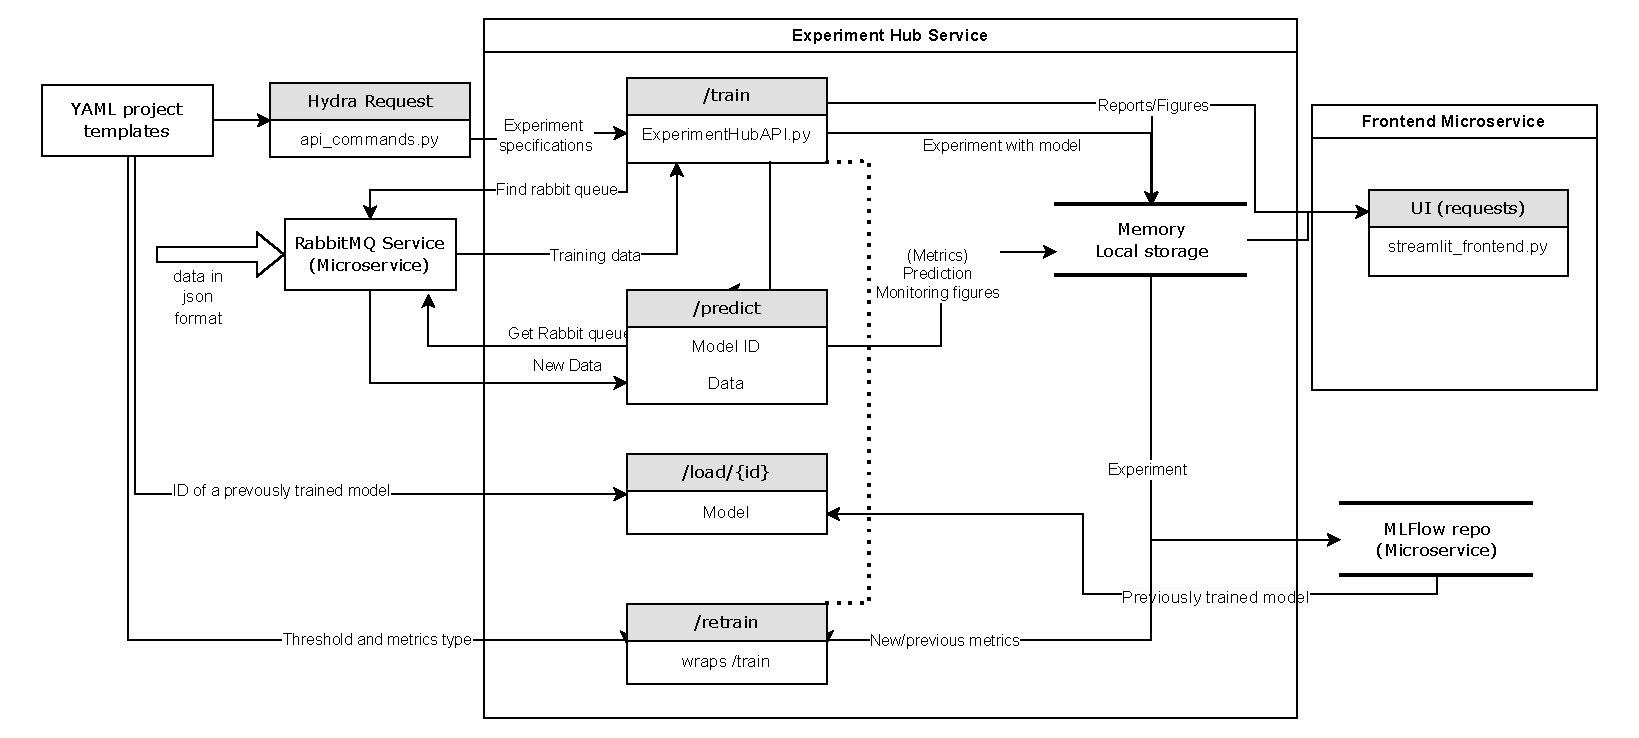
\includegraphics[width=0.9\textwidth, clip, trim={0 0 0 0}]{figs/api_arch.pdf}
\caption{System Architecture}
\label{fig1}
\end{figure}


An MLflow repository is \textbf{required} to execute the REST API commands of the ExperimentHub. This microservice contains the Experiment names (queue names of the RabbitMQ service), under which several run IDs are accessable. Individual models are saved in a standardized format with a run ID under the corresponding queue name. As such, any instance of ExperimentHub will be able to reload models. We have not yet integrated the MLflow registry with the package yet.


% The architecture is designed for easy modification and extensibility. Users can enhance functionality by adding REST API commands to the ExperimentHub service and integrating additional microservices through Docker Compose. For example, Grafana and Prometheus can be incorporated for system monitoring, PostgreSQL can be installed to save out the incoming data and the results, while Nginx can be deployed for efficient load balancing. This modular design allows seamless customization to meet diverse operational needs, although it may require some manner of modifications first to the ExperimentHub Service.


The architecture commands in ExperimentHubAPI provide a comprehensive interface to manage experiments, models, and data workflows. These commands enable users to perform critical tasks such as training, saving, loading, and predicting with models, as well as retrieving configurations and visualizations. Table \ref{restapi_commands} summarizes the available commands and their functionalities.
\begin{table}[h!]
\caption{API Commands in ExperimentHubAPI.py}
\label{restapi_commands}
\centering
\small % Added for better fit
\begin{tabular}{|p{0.35\textwidth}|p{0.1\textwidth}|p{0.5\textwidth}|}
\hline
\textbf{Endpoint} & \textbf{HTTP Method} & \textbf{Description} \\
\hline
/ & GET & Default path. Returns a "Hello World" message. \\
\hline
/flush/\{queue\} & POST & Removes all data from the specified RabbitMQ queue. \\
\hline
/\{name\}/train & POST & Starts training for the specified experiment, setting up the training configuration. Requires data in the Rabbit queue and a configuration file.\\
\hline
/\{name\}/load & POST & Loads an experiment by its name. \\
\hline
/\{name\}/load/\{run\_id\} & POST & Loads an experiment using the specified run ID from MLflow. \\
\hline
/\{name\}/save & POST & Saves the current experiment to the MLflow server. \\
\hline
/\{name\}/predict & POST & Initiates a prediction call for the specified experiment. Requires a request and data in the RabbitMQ queue \{name\}. \\
\hline
/\{name\}/plot/\{plot\_name\} & GET & Returns a plot (figure) for the specified experiment and plot name in JSON. \\
\hline
/\{name\}/plot\_eda/\{plot\_name\} & GET & Returns the EDA plot (figure) for the specified experiment and plot name in JSON. \\
\hline
/\{name\}/train\_data & GET & Returns training data for the specified experiment in JSON. \\
\hline
/\{name\}/cfg & GET & Returns the configuration details of the specified experiment. \\
\hline
/experiments & GET & Lists all experiment names and available figure names. \\
\hline
/\{name\}/run\_id & GET & Returns the run ID (MLflow) of the specified experiment. \\
\hline
/\{name\}/exp\_id & GET & Returns the experiment ID (MLflow) of the specified experiment. \\
\hline
/\{name\}/retrain & POST & Starts retraining an experiment as requested. \\
\hline
\end{tabular}
\end{table}

When data is sent to ExperimentHub, REST API commands can be used to access specific processes. For a new model, the process begins by sending a training dataset to the RabbitMQ queue and then submitting a training configuration via the /\{name\}/train API call. This command initiates model training. If the training completes without exceptions, the model is saved to the experiment in MLflow for future use and provides information about the training process on the frontend to check if the model is viable.

For example, if sensor data lacks labels, a fault detection experiment can be conducted using methods like DBSCAN. Each implemented model includes a predict function that updates its figures to better represent the data it has processed. Using the /\{name\}/predict API call, the system retrieves data from the queue, updates the current results (\textit{e.g. anomalies shown by DBSCAN}, and displays them on the frontend. Both the train and predict calls return detailed information about the outcomes of the REST API operations.


Additional commands enhance functionality, such as saving to and loading from MLflow, or retraining to replace the current model in the ExperimentHub. Automated retraining can also be configured during the training phase, enabling continuous model updates based on new data or predefined conditions.



% \todo[inline]{Implement /results! Implement /kill! Better description formatting}

The project template is structured to facilitate the creation and management of machine learning experiments. The configs (hydra templating) folder contains configuration files for specific ID-s that define experiment functions, parameters, and model settings. The config.yaml file in particular plays a central role by coordinating multiple experiments. 
The config.yaml is used to compose a configuration file with relevant information to send to the ExperimentHub, which upon retrieval, builds the models. It dynamically pulls data from different RabbitMQ queues (keys in the config.yaml) for each experiment, allowing for the execution of several tasks with different configurations. This setup enables users to train and test various models using diverse datasets, streamlining the management of complex workflows and facilitating scalable experimentation, without redeploying the Docker image. For example:
\begin{listing}[ht]
\begin{minted}[
    gobble=4,
    frame=single,
    linenos
  ]{yaml}
    defaults:
     - pump : DBSCAN.yaml # pump is the ID of the experiment and 
     #queue name for rabbit and DBSCAN is the name for the config to use
     # the configuration is a set of instructions for the experiments.
\end{minted}
\caption{Project template for multiple model configuration definition. Keyword "defaults" must contain a list of \{ID\} for folder, which denotes RabbitMQ queue name and experiment name, and \{name\}.yaml for the configuration in folder \{ID\} describing model information. The Hydra package helps compose the necessary Hydra files, and can be used to select several models from existing configurations depending on the Operator needs.}
\label{lst:proj_temp}
\end{listing}


The configuration file in Listing \ref{lst:proj_temp} will configure the ExperimentHub to pull data from queue "pump", name the experiment to "pump" and use the DBSCAN.yaml configuration to train a DBSCAN model. This requires a living RabbitMQ connection with data in the queue and a "/\{name\}/train" post request as the ExperimentHub acts on a Remote Procedure Call principle (requires a request to call for pulling the data, and will communicate if it succeeded). In this case, \{name\} variable can be thought of as DBSCAN.


The \{name\}.yaml file plays a critical role in the framework by serving as the configuration backbone for experiments and their models. An example for the DBSCAN is provided in Listing \ref{lst:exp_temp}. It defines key functions of the Experiment (abstract) class to be called, such as the module and experiment type (\textit{load\_object}), dataset details (setup), and model configurations (\textit{create\_model}). By encapsulating settings in a structured format, it allows for dynamic and modular management of machine learning workflows, enabling users to adapt the system to various datasets and models without altering core code. This ensures flexibility, reproducibility, and streamlined experimentation. To configure the DBSCAN model for fault detection, the \{name\}.yaml file must specify the correct experiment module and class name under the \textit{load\_object} section. The setup section requires a column name for the timestamp indicator. Under the \textit{create\_model} section, the DBSCAN algorithm is selected by setting model: "dbscan". Key parameters such as \textit{eps} (maximum neighborhood distance) and \textit{min\_samples} (minimum points required to form a cluster) are also defined in the configuration files.

Example for the DBSCAN configuration file:
\begin{listing}[ht]
\begin{minted}[
    gobble=4,
    frame=single,
    linenos
  ]{yaml}
    load_object:
      module: framework.FaultDetection ## Experiment .py file
      name: FaultDetectionExperiment # Class name of the experiment
    
    setup:
      datetime_column: "timestamp" # Column representing time;
      #MUST NOT have a 'data' keyword
    eda:
    create_model:
        model: "dbscan" # DBSCAN clustering for fault detection
        params:
          eps: 2 # Maximum distance between points in a neighborhood
          min_samples: 5 # Minimum number of points to form a cluster
\end{minted}
\caption{Experiment template for specifying a model. Each keyword represents a function in the experiment. The parameters are dynamically loaded from the config file to the Experiment class, which in turn will call these functions during the /\{name\}/train API call.}
\label{lst:exp_temp}
\end{listing}
Which can be used to train a DBSCAN model. One can also use the "/\{name\}/predict" command to pull data from rabbit and use the model on unknown data.

\textbf{It is important to note that models retain their inherent properties as this system provides an infrastructure for data and use rather than reimplementing these methods.}


 \subsection{Software functionalities} \label{framework}
While MLflow is designed to be framework-agnostic, its reliance on flavors introduces some framework-specific dependencies. This can result in a difference of the approach taken to integrate models from certain frameworks. Of course, the MLflow contains pyfunc general approach to models, however it has a lack of convenience functions, and such this limitation creates challenges when integrating models. Therefore, the framework limits the use of models to custom sklearn models, which are derived from \textit{BaseEstimator} class.


The Experiment class serves as the core of the ExperimentHub system, managing the lifecycle of machine learning experiments, including tasks such as training, saving, loading, and predicting. This class holds essential metadata about each experiment, \textit{e.g.} its configuration, plots, and the corresponding RabbitMQ queue name. Figure \ref{fig2} presents the interaction between the Experiments and the models and general methods that need to be implemented.

\begin{figure}[!h]
\centering
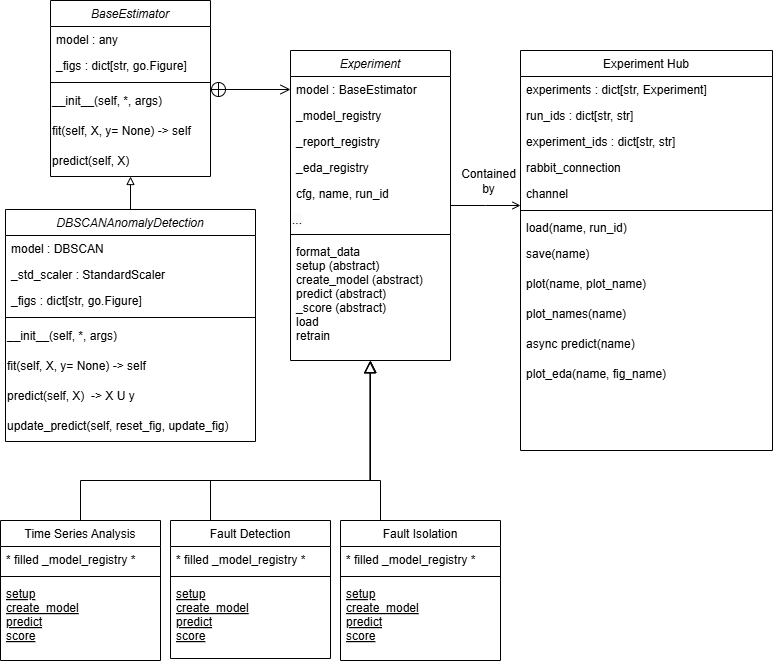
\includegraphics[width=0.8\textwidth, clip, trim={0 0 0 0}]{figs/class_interactions.png}
\caption{\textbf{Class interactions.} Empty-headed arrows show that an object implements a target abstract class.}
\label{fig2}
\end{figure}

% \todo[inline]{Furcsa így ez a figure 3, dbscan bemegy a baseestimatorba, lent meg a 3 féle mód van, de dbscan csak fault detection ... 
% part of 0...1...0 azok mik a nyílon? -- Az ULM-ben az üres nyilak implementálást jelenti, a keresztezett kör pedig azt mutatja, hogy a részét képezi. Javítottam a 010 részt, nem lényeges. Még javítani a nyilak irányán}

Derived classes extend the functionality of the Experiment class by providing specialized behaviors tailored to specific types of experiments or workflows. These subclasses implement custom methods for model training processes, prediction, or experiment management tasks. For example, one method might handle specific pre-processing steps for certain datasets, while another might focus on hyperparameter tuning or anomaly detection. These derived classes enhance the flexibility and modularity of the ExperimentHub system, enabling users to modify the behavior of experiments to meet their requirements. Table \ref{experiment_funcs} provides information on which functions are to be overloaded, and which are convenience functions integrated with the ExperimentHub. An experiment is derived from Experiment abstract base class.


The framework includes default implementations of the Experiment class to address various use cases. Fault Detection is designed for anomaly detection, aiming to identify errors in production, such as incorrect packaging selections or failed resource placements. As a multivariate approach, it can group production inputs and provide insights into which sensors might be contributing to the problem. It supports multiple sensors and does not require labeled output, making it versatile for detecting anomalies in complex systems.

The Fault Isolation class serves as a broader wrapper for classification problems where labeled data is available. It is particularly useful for root cause analysis, identifying sensor contributions to anomaly detection, and analyzing machine states. This facilitates a deeper understanding of the system and supports targeted troubleshooting and optimization.

Time Series Analysis class is designed for monitoring sensor data over time, offering insights into the behavior of individual sensors across their lifecycle. It is ideal for applications like predictive maintenance and real-time monitoring, enabling proactive system management and minimizing unexpected downtime.

%\todo[inline]{Ez a process mining csak random megjelent, úgyhogy kiemelném egy átvezetővel, hogy nem direktbe a pred. karbantartás eszközéhez tartozik, de implementálva van folyamatfeltárás - ok-okozati összefüggések feltárása céljából ... }
If the data is not tabular or nominal, the process mining may help analyze otherwise unusable data. Process Mining class is a straightforward implementation of process mining techniques, which can also find casual connection in between sequences and states. These approaches can be applied to analyze operator behavior and machine logs, offering valuable insights into system workflows and identifying potential areas for improvement.


% \begin{table}[h!]
% \caption{Anatomy of an Experiment class}
% \centering
% \resizebox{\textwidth}{!}{ % Scale table to fit text width
% \scriptsize % Even smaller text
% \setlength{\tabcolsep}{2pt} % Minimal column spacing
% \begin{tabular}{|l|c|p{3.8cm}|p{3.8cm}|}
% \hline
% \textbf{Function Name} & \textbf{Overloadable} & \textbf{Description} & \textbf{Notes} \\
% \hline
% \texttt{\_\_init\_\_} & \checkmark (must be defined) & Loads model classes, and sets up requirements for the Experiment to work & Must be defined is a strict format for each Experiment \\
% \hline
% \texttt{setup} & \checkmark (must be defined) & Sets up the experiment, must be implemented by the child class. & Defines the initial setup for running experiments. \\
% \hline
% \texttt{create\_model} & \checkmark & Trains the model, must be implemented by the child class. & Models should be defined here. \\
% \hline
% \texttt{predict} & \checkmark & Predicts the target variable, must be implemented by the child class. & Requires test data input. \\
% \hline
% \texttt{\_score} & \checkmark & Calculates the metrics of the model, must be implemented by the child class. & Evaluates model performance. \\
% \hline
% \texttt{format\_data} & \checkmark (caution) & Formats data from JSON to a \texttt{DataFrame}. & Converts raw data into a usable format. \\
% \hline
% \texttt{plot\_model} & x & Plots model visualizations using stored figures. & Visualizes the model's results. \\
% \hline
% \texttt{save} & x & Saves the experiment (model, reports, and metadata). & Essential for persisting the experiment state. \\
% \hline
% \texttt{load} & x & Loads an experiment including model and reports. & Restores the saved experiment state. \\
% \hline
% \texttt{convert\_datetime} & \checkmark (caution) & Converts date/time columns to the desired format. & Necessary for handling time-based data. \\
% \hline
% \texttt{eda} & x & Performs exploratory data analysis (EDA) on training data. & Helps in understanding the dataset's properties. \\
% \hline
% \texttt{retrain} & \checkmark & Checks whether retraining is necessary based on metrics. Can be overloaded if a new logic is required. & Ensures that the model is always up-to-date. \\
% \hline
% \texttt{spc} & x & Creates statistical process control (SPC) charts (WIP). & Work in progress for statistical analysis. \\
% \hline
% \texttt{run} & x & Runs the experiment, orchestrates setup and training. & Entry point for running the entire experiment pipeline. \\
% \hline
% \texttt{join\_data} & x & Combines old and new data, applies retrain window logic. & Useful for incremental learning. \\
% \hline
% \texttt{export} & x & Exports reports as HTML and logs them to MLflow. & Facilitates report generation and tracking. \\
% \hline
% \texttt{get\_eda\_reports} & x & Retrieves available EDA report IDs. & Helps access previously generated EDA reports. \\
% \hline
% \texttt{get\_fig\_types} & x & Retrieves available figure IDs from the model. & Useful for retrieving model-specific visual outputs. \\
% \hline
% \texttt{load\_object} & x & Dynamically loads a class or function from a module. & Enables dynamic loading of components. \\
% \hline
% \end{tabular}
% }
% \label{experiment_funcs}
% \end{table}


% An Experiment class contains model classes from which it can instantiate and train models. The extension requires the modification of the experiment class. It is the future work of the authors to improve the package for dynamic import of models.

Table \ref{imp_models} contains the list of models implemented in the framework. The \textit{setup} function handles the data formatting, \textit{create\_model} uses a predefined model training process, along with \textit{predict} that infers new results from the model. Both function requires a string-like input that is most often a read json from the RabbitMQ. During the definition of the class, only models with similar data input requirements can be used. Some functions may be reconfigurable, but it is hard to debug properly. Table \ref{imp_models} provides the list of models and their libraries.
%\textit{\_score}
\begin{table}[h!]
\caption{\textbf{Models included in the Framework.} The columns focus on the implemented models (from BaseEstimator class), experiment types, and associated packages}
\centering
\small % Reduced font size for better fit
\begin{tabular}{|l|l|l|}
\hline
\textbf{Model Name} & \textbf{Experiment Type} & \textbf{Package} \\
\hline
Decision Tree & Fault Isolation & scikit-learn \citep{scikit-learn} \\
\hline
Random Forest & Fault Isolation & scikit-learn \citep{scikit-learn} \\
\hline
Naive Bayes & Fault Isolation & scikit-learn \citep{scikit-learn} \\
\hline
Hidden Markov Models & Fault Isolation & hmmlearn \citep{hmmlearn} \\
\hline
Bayesian Network & Fault Isolation & pgmpy \citep{Ankan2015} \\
\hline
Markov Chain & Fault Isolation & statsmodels \citep{seabold2010statsmodels} \\
\hline
PCA & Fault Detection & pca \citep{Taskesen_pca_A_Python_2020} \\
\hline
DBSCAN & Fault Detection & scikit-learn \citep{scikit-learn} \\
\hline
Elliptic Envelope & Fault Detection & scikit-learn \citep{scikit-learn} \\
\hline
Isolation Forest & Fault Detection & scikit-learn \citep{scikit-learn} \\
\hline
ARIMA/SARIMA & Time Series Analysis & statsmodels \citep{scikit-learn} \\
\hline
LSTM & Time Series Analysis & TensorFlow \citep{tensorflow2015-whitepaper} \\
\hline
Autoencoder & Time Series Analysis & TensorFlow \citep{tensorflow2015-whitepaper} \\
\hline
Prophet & Time Series Analysis & Prophet \citep{prophet} \\
\hline
SSA & Time Series Analysis & pySSA \citep{pySSA} \\
\hline
Heuristics Miner & Process Mining & pm4py \citep{pm4py} \\
\hline
Top-K Rules & Process Mining & SPMF \citep{fournier2016spmf} \\
\hline
Apriori Association Rules & Process Mining & SPMF \citep{fournier2016spmf} \\
\hline
CMSPAM & Process Mining & SPMF \citep{fournier2016spmf} \\
\hline
\end{tabular}
\label{imp_models}
\end{table}

For defining your own models, what you require is the \textit{BaseEstimator} from sklearn and how the data is passed to the model in the experiment class. Listing \ref{lst:new_model} provides an abstracted, high level overview example for creating a model. \_figs attribute, \_\_init\_\_, fit, predict, update\_predict functions must be defined if we want to use this example model for Fault Detection.  For the prediction, the incoming data is a dataframe that is expanded with the results and return at the end of the prediction.
 
\begin{listing}[ht]
\begin{minted}[frame=single, fontsize=\small, linenos]{python}
class EXAMPLEAnomalyDetection(BaseEstimator):
    """Strictly follow sklearn API!""""
    _model: MODELTYPE = None
    _std_scaler: StandardScaler = None
    _figs: dict[str, go.Figure] = {} # must have!
    def __init__(self, *, param1=2, param2=None):
        """Set the parameter for fitting and prediction"""
        self.param1 = param1 # set parameters
        self.param2 = param2
        self._std_scaler = StandardScaler() # make scaler, use internally
    def fit(self, X, y=None):
        """Creates a instance of the class based on the given dataset"""
        self.scheme = X.columns # should be present
        sc_X = self._std_scaler.fit_transform(X)
        self._model = MODELTYPE(param1, param2).fit(sc_X)
        self.anomalies = self._model.labels_ == -1 
        ## for the sake of simplicity, -1 is an anomaly
        ##Create predict figures in _fig
        self.update_predict(X, reset_fig=True, update_fig=False)
        self.is_fitted_ = True
        return self
    def predict(self, X):
        """This function applies scaling and adds a new anomalies column"""
        sc_X = self._std_scaler.transform(X)
        nX = X.copy()
        nX["outliers"] = self._model.fit_predict(sc_X) == -1
        return nX
    def update_predict(self, X, reset_fig=False, update_fig=True):
        if reset_fig: # for each column
            for i, col in enumerate(self.scheme):
                self._figs[f"{col}_predict"] = make_subplots(
                    rows=1, cols=1, subplot_titles=("Prediction",))
                self._figs[f"{col}_predict"].update_xaxes(
                    title_text='Index', row=1, col=1)
                self._figs[f"{col}_predict"].update_yaxes(
                    title_text=col, row=1, col=1)
                self._figs[f"{col}_predict"].update_layout(
                    title_text=f'Outlier prediction for {col}', showlegend=False)
        if update_fig:
            for i, col in enumerate(self.scheme):
                self._figs[f"{col}_predict"].add_trace(
                    go.Scatter(x=X.index, y=X.loc[:, col], mode='lines', name=col, 
                               line=dict(color='blue')), row=1, col=1
                )
                self._figs[f"{col}_predict"].add_trace(
                    go.Scatter(x=X.index[X["outliers"]], y=X.loc[X["outliers"], col], 
                               mode='markers', name='Outliers',
                               marker=dict(color='red')),
                               row=1, col=1)
\end{minted}
\caption{Experiment template for specifying a model. Each keyword represents a function in the experiment. The parameters are dynamically loaded from the config file to the Experiment class, which in turn will call these functions during the /\{name\}/train API call.}
\label{lst:new_model}
\end{listing}


  \clearpage
%  \subsection{Sample code snippets analysis (optional)}
% \todo[inline]{add DBscan example here!}
% \clearpage
\section{Illustrative examples}

In order for the application to work properly, one needs to set up the docker environment. Listing \ref{lst:app_only} provides commands to pull the application from DockerHub:

\begin{listing}[h!]
\begin{minted}[
    gobble=4,
    frame=single,
    linenos
  ]{console}
    docker pull rabbitmq:3.12.14-management-alpine 
    docker pull ipkovichadam/observml:mlflow
    docker pull ipkovichadam/observml:backend
    docker pull ipkovichadam/observml:frontend
    docker compose up
    \end{minted}
\caption{Docker compose up without installing dependencies.}
\label{lst:app_only}
\end{listing}

In case of customizing and improving the framework, it might be one's best interest to set up local services without having to create a Docker Image. Listing \ref{lst:local_app} presents a local approach that helps you develop new experiments and models. 

\begin{listing}[h!]
\begin{minted}[
    gobble=4,
    frame=single,
    linenos
  ]{console}
    poetry install
    mlflow run
    docker run --publish 5672:5672 rabbitmq:3.12.14-management-alpine
    python ExperimentHubAPI.py
    streamlit run streamlit_frontend.py
\end{minted}
\caption{Local use of the application (\textit{e.g.} for development). Use each command on a different terminal}
\label{lst:local_app}.
\end{listing}



Figure \ref{empty_hub} presents the default user interface for the Experiment Hub. On the sidebar, two modes are possible; one for presenting the exploratory data analysis, and one for monitoring (training and prediction results). A slider is available to set the refresh duration, which can reduce the strain on the front-end application. The Experiment tab expands upon new models, currently there is no model to select. On the right-hand side the relevant EDA figures can be selected, which is also filled if new models are trained to show the figures of the selected experiment. This is only an example UI, which provides example code on how to communicate with the backend API and can be replaced by custom UIs such as Graphana or Promethean.

\begin{figure}[h!]%
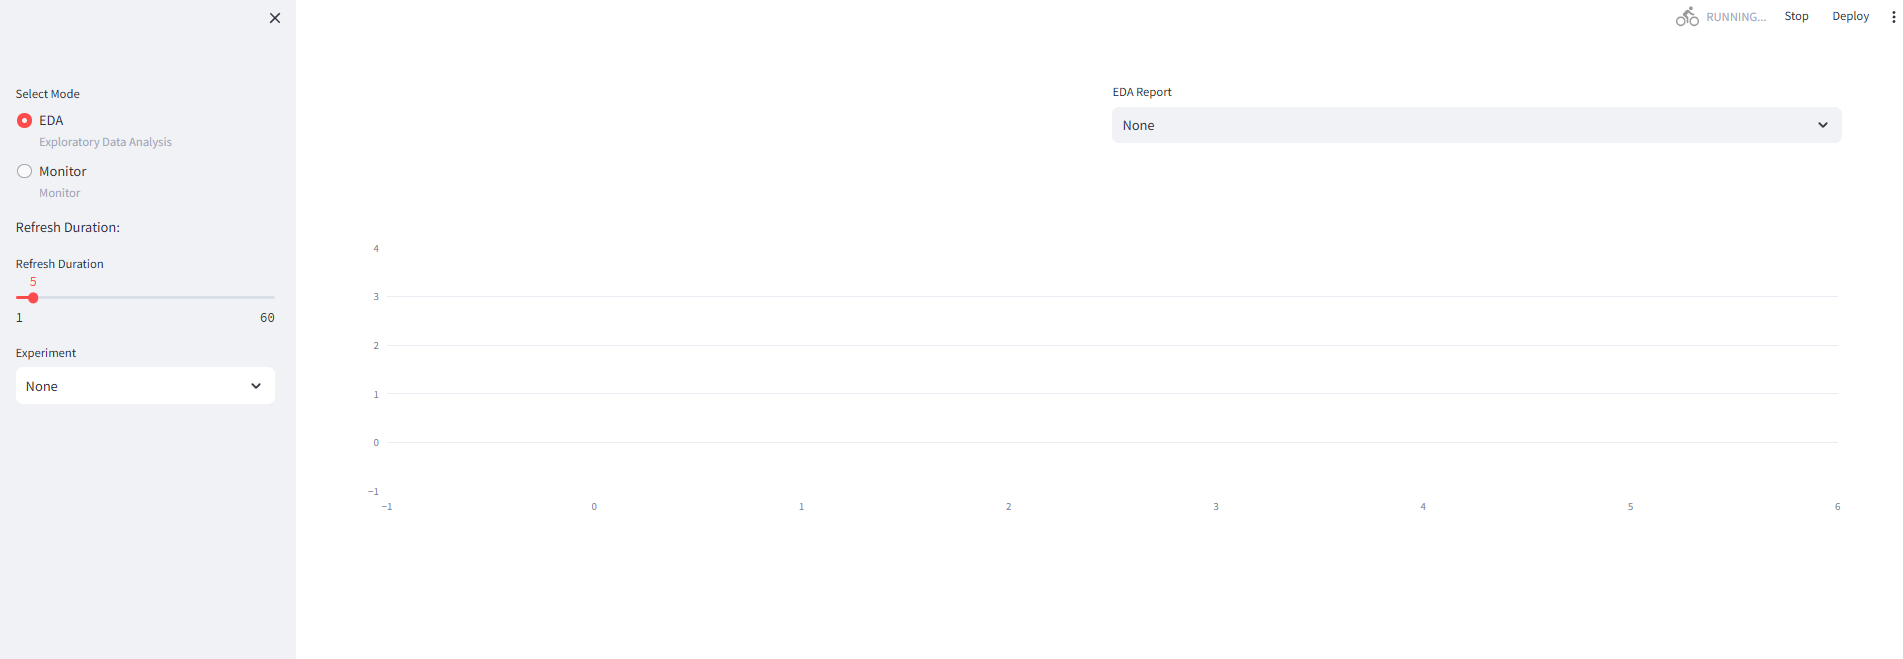
\includegraphics[width=0.9\textwidth, clip, trim={0 0 0 0}]{figs/empty_hub.png}
{\caption{User Interface for an empty ExperimentHub.}
\label{empty_hub}}
\end{figure}


To train models, we are required to post a train request, and push a dataset to the rabbit. Some example codes are provided.

% \subsection{Fault Isolation - Decision Tree} \label{res:fi}

% If dataset provides labels or identification related data, then it is possible to use fault isolation to uncover specific states a machine could be in. This may be important as some sensors never deviate from the expected value in a well-defined state. For example, electrical lines with 3 phase electricity also requires proper monitoring to ensure seamless service \citep{circuitdata}. The output should always be one, however there are cases, when anomaly happens and alters the state of the network, the output returns zero. In this case, we apply the framework to build a decision tree model and provide monitoring results for incoming data. The dataset contains information on the Output and the three voltages (Va, Vb, Vc) and three currents (Ia, Ib, Ic), and was split to one training, and eight predict function test sets for the case study. The list \ref{lst:decision_tree} depicts the instance of the configuration file that is used to generate the results.

% \begin{listing}[h!]
% \begin{minted}[
%     gobble=4,
%     frame=single,
%     linenos
%   ]{yaml}
%     load_object :
%       module: framework.FaultIsolation
%       name: FaultIsolationExperiment
%     setup:
%         datetime_column : ds
%         datetime_format : "ms" 
%         predict_window : 
%         ## how much samples to show during prediction. if empty, it will show all.
%         target : "Output (S)"
%         #retrain :
%           #retrain_window : 5000 
%           ## if none, retrain on all data.
%           #metric : "Accuracy"
%           ## depending on experiment -> Accuracy, F1, Precision, Recall
%           #metric_threshold : 0.9 
%           ## if we get this, retrain
%           #higher_better : True
%           ## less or more if this threshold is bad performance?
%     eda:
%     create_model :
%         model : "dt" #"ee" #"dbscan" #"pca"
%         params:
% \end{minted}
% \caption{Configuration file for Decision Tree-based fault isolation.}
% \label{lst:decision_tree}.
% \end{listing}

% By running adding the dataset into data.yaml, and running train\_local\_script.py, we obtain the results of the training. The system automatically provides an EDA, in this case, a correlation matrix is depicted in \ref{fi:corr}.

% \begin{figure}[h!]%
% \FIG{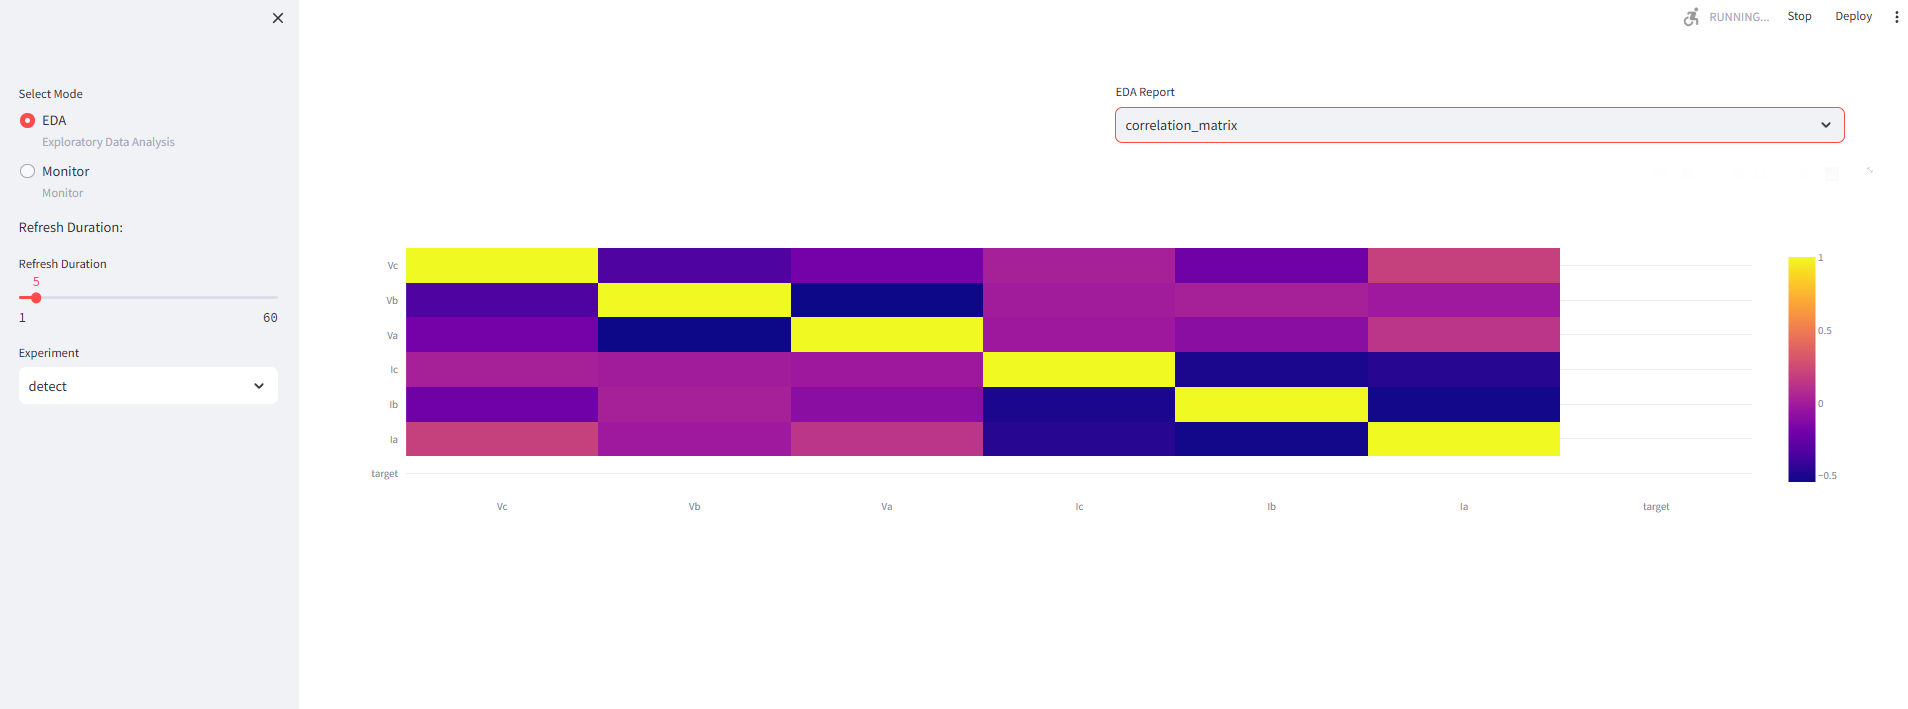
\includegraphics[width=0.9\textwidth, clip, trim={0 0 0 0}]{Figs/fi_eda.png}}
% {\caption{EDA for Decision Tree model, correlation matrix. "target" is the output, and since it is a label, correlation is not calculated}
% \label{fi:corr}}
% \end{figure}


% One can observe the performance of the method in the "Monitor" mode. Figure \ref{fi:conf} depicts the confusion matrix of the decision tree.

% \begin{figure}[h!]%
% \FIG{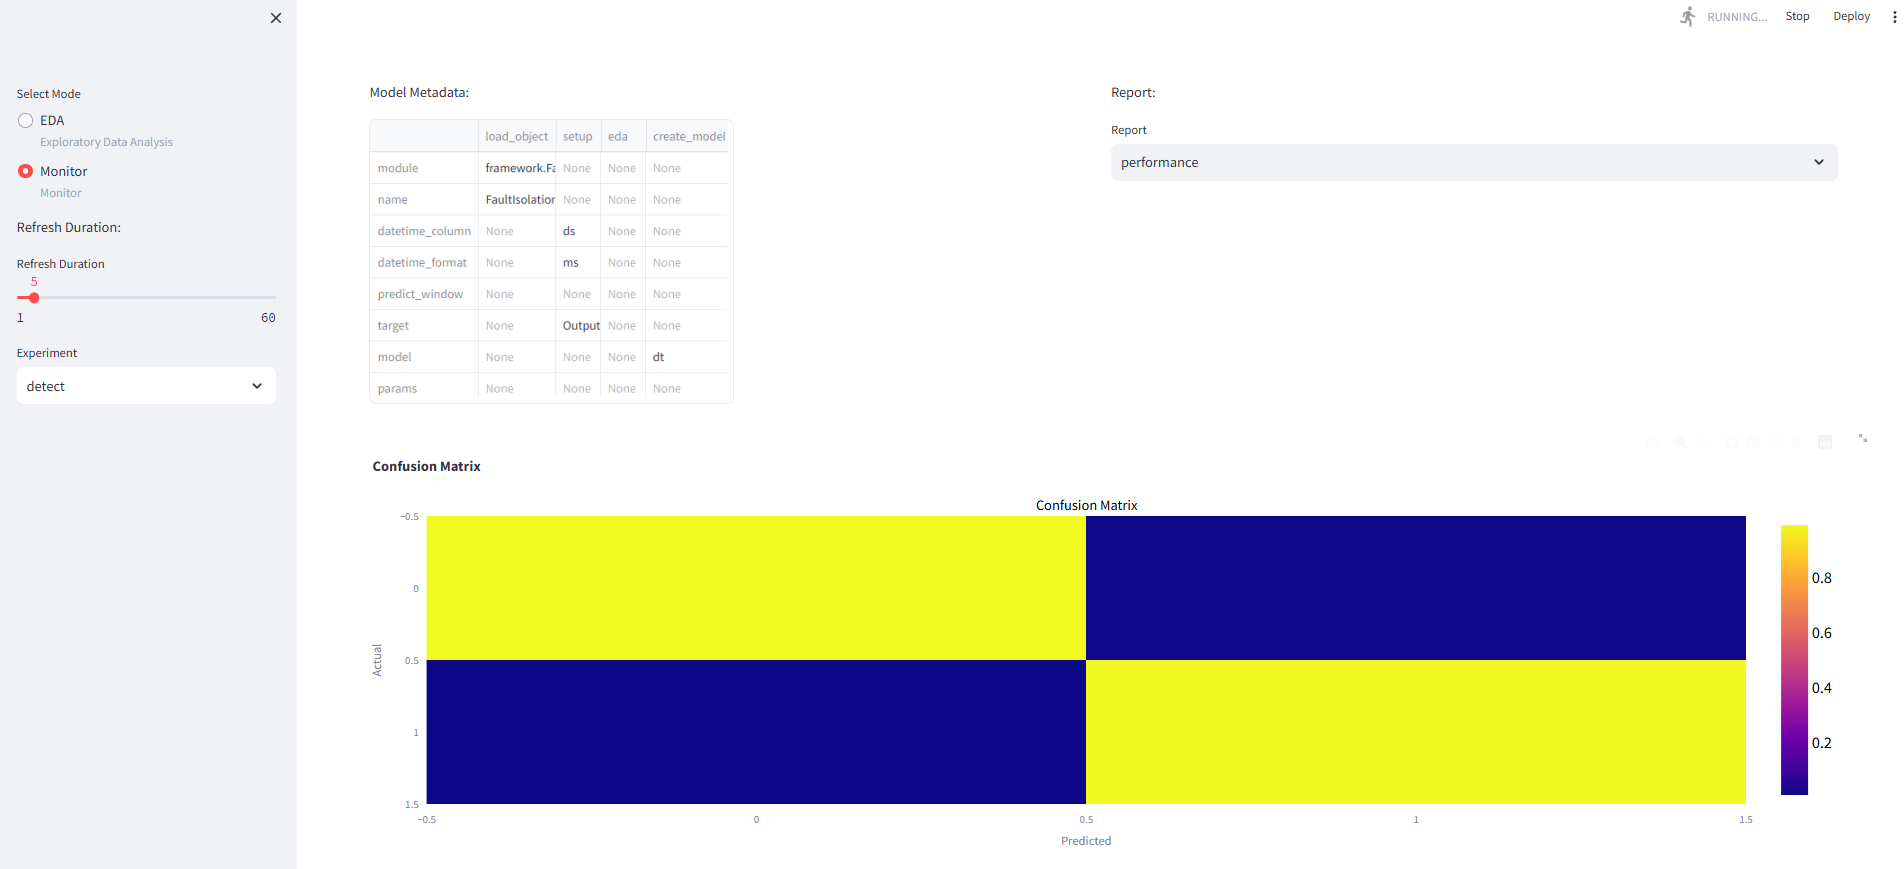
\includegraphics[width=0.9\textwidth, clip, trim={0 0 0 0}]{Figs/confusion_mat.png}}
% {\caption{Confusion matrix for Decision Tree model trained on electrical transfer data}
% \label{fi:conf}}
% \end{figure}


% Model objects can create custom figures, and as such, there are unique functionalities depending on the configuration files. In this case, decision tree model contains a feature importance function that is shown in Figure \ref{fi:import}.

% \begin{figure}[h!]%
% \FIG{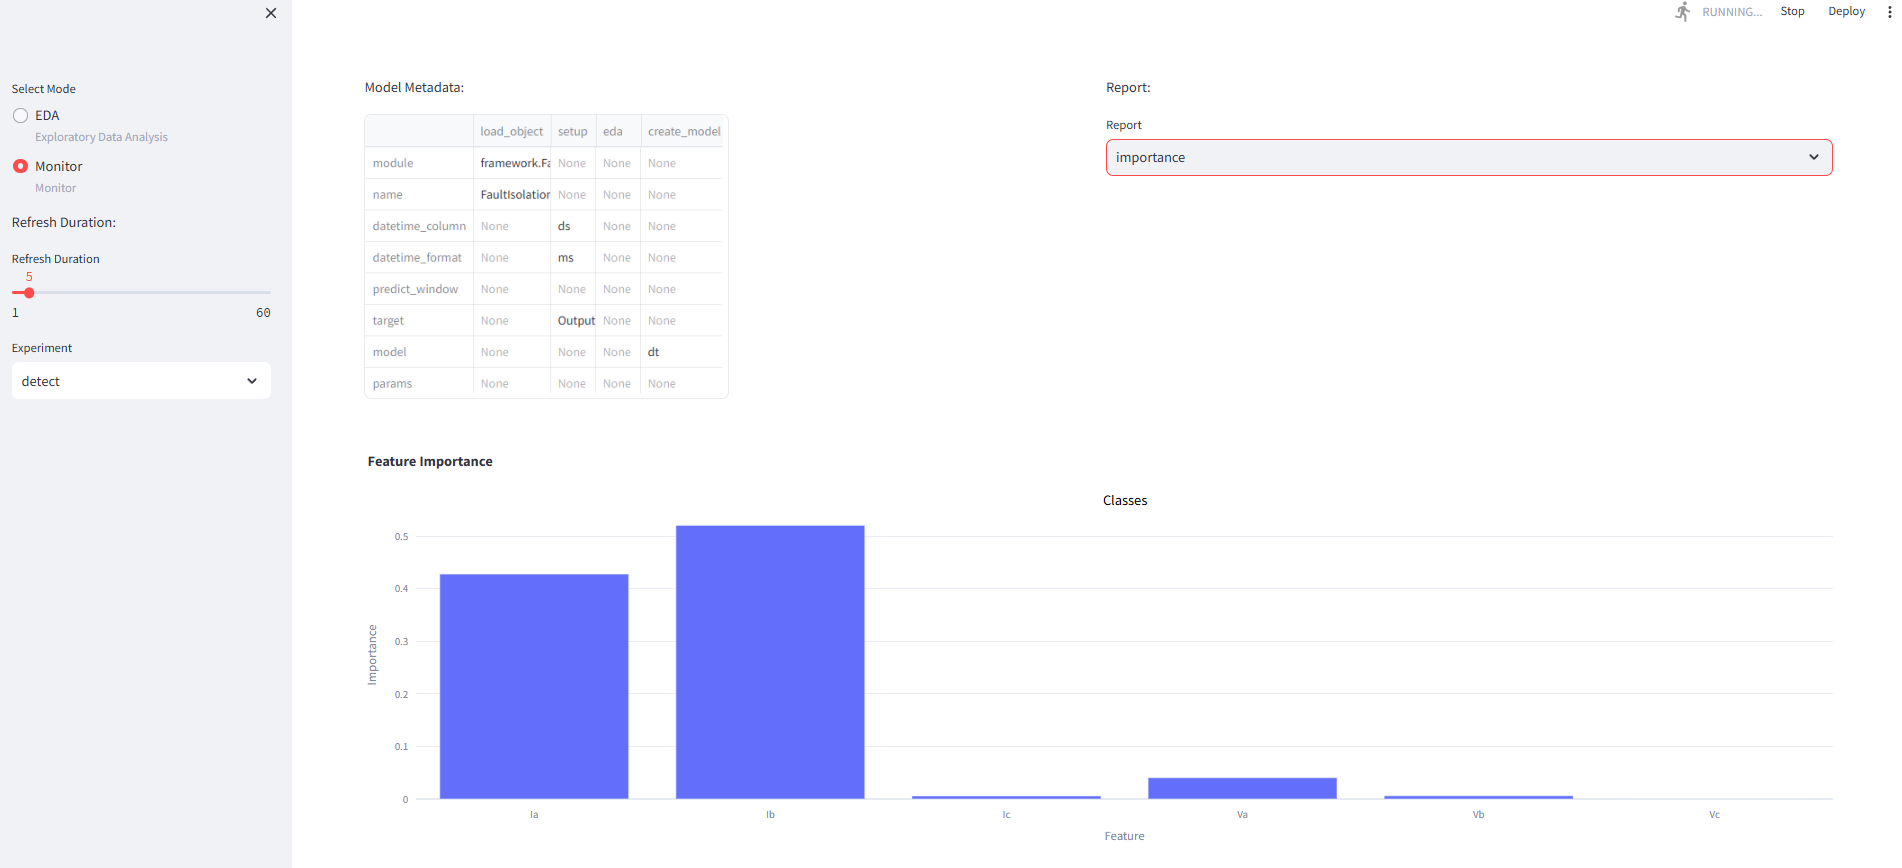
\includegraphics[width=0.9\textwidth, clip, trim={0 0 0 0}]{Figs/fi_importance.png}}
% {\caption{Feature importance of the currents and voltages against the output}
% \label{fi:import}}
% \end{figure}


% From the importance analysis, one can derive that Ib contains significant information about the output variable. Therefore, Figure \ref{fiibclass} visualizes the dataset and shows the respective states (normal/faulty).

% \begin{figure}[h!]%
% \FIG{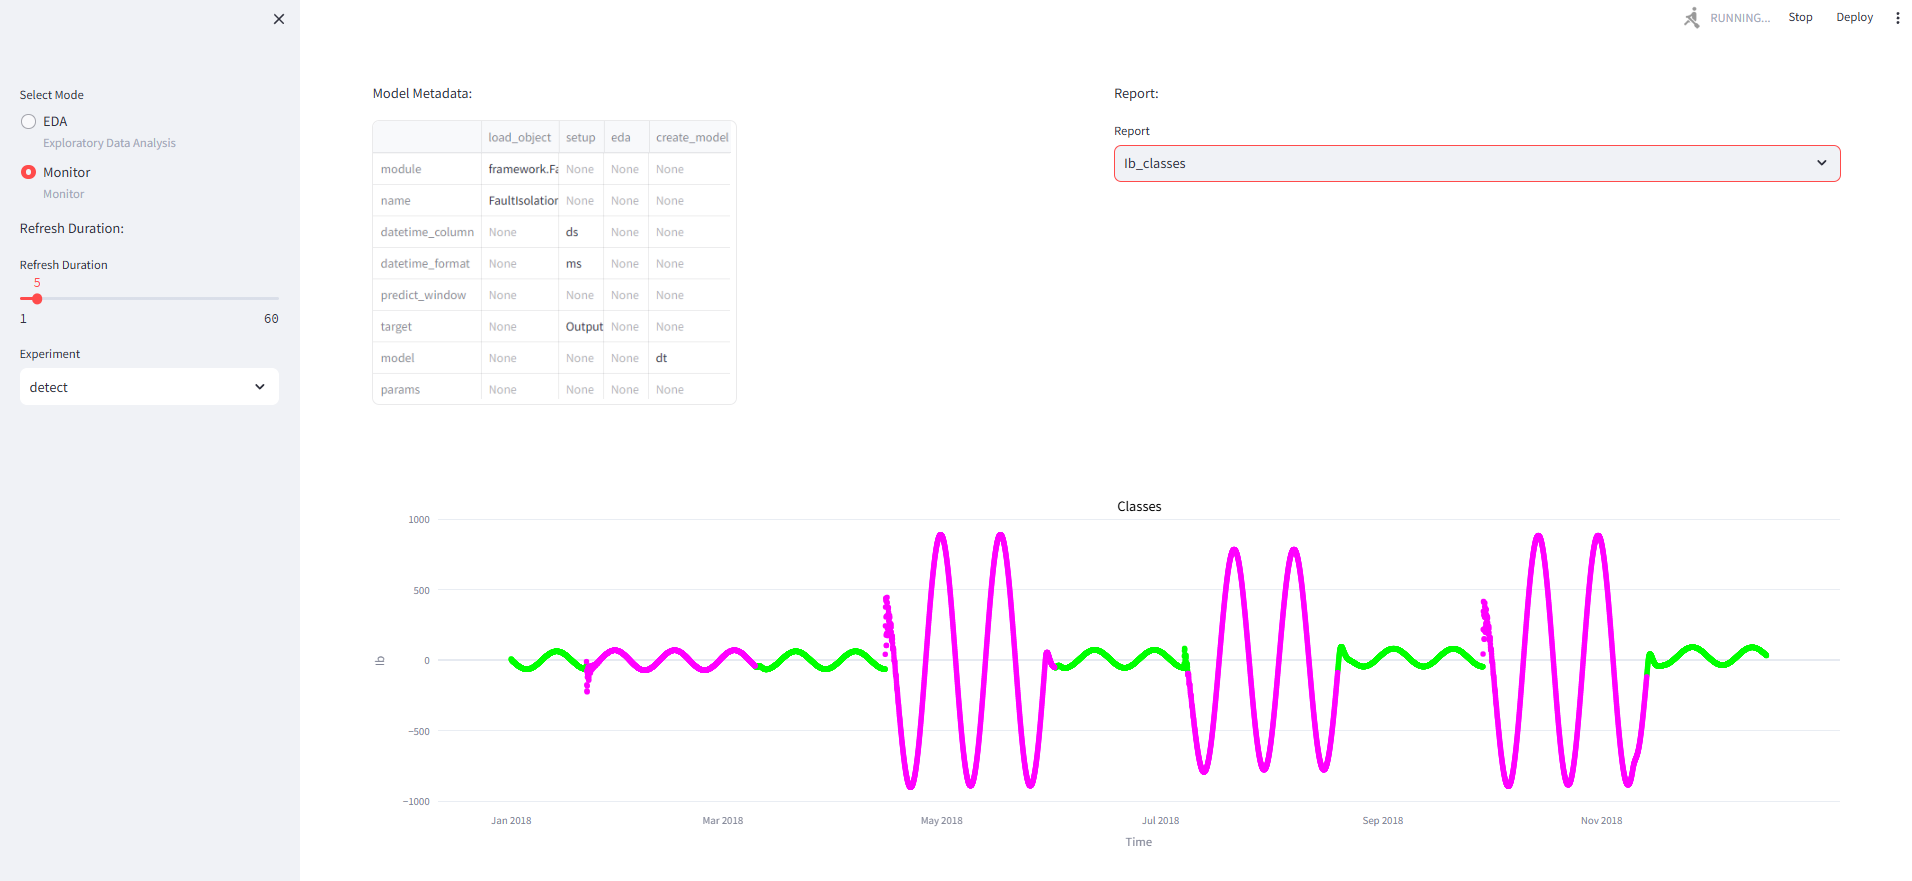
\includegraphics[width=0.9\textwidth, clip, trim={0 0 0 0}]{figs/fi_class.png}}
% {\caption{Ib classes assigned for training. Purple/pink denotes on, while green presents off state}
% \label{fiibclass}}
% \end{figure}


% There is also an option to check the metrics of the model. It is possible that data drift happens during monitoring, and so the model must be retrained to keep the accuracy. If we request prediction from the backend (with test\_script.py) for 8 consecutive data snippet, we will obtain Figure \ref{fi_metrics} to present performance metrics on the dashboard.


% \begin{figure}[h!]
% \centering
% 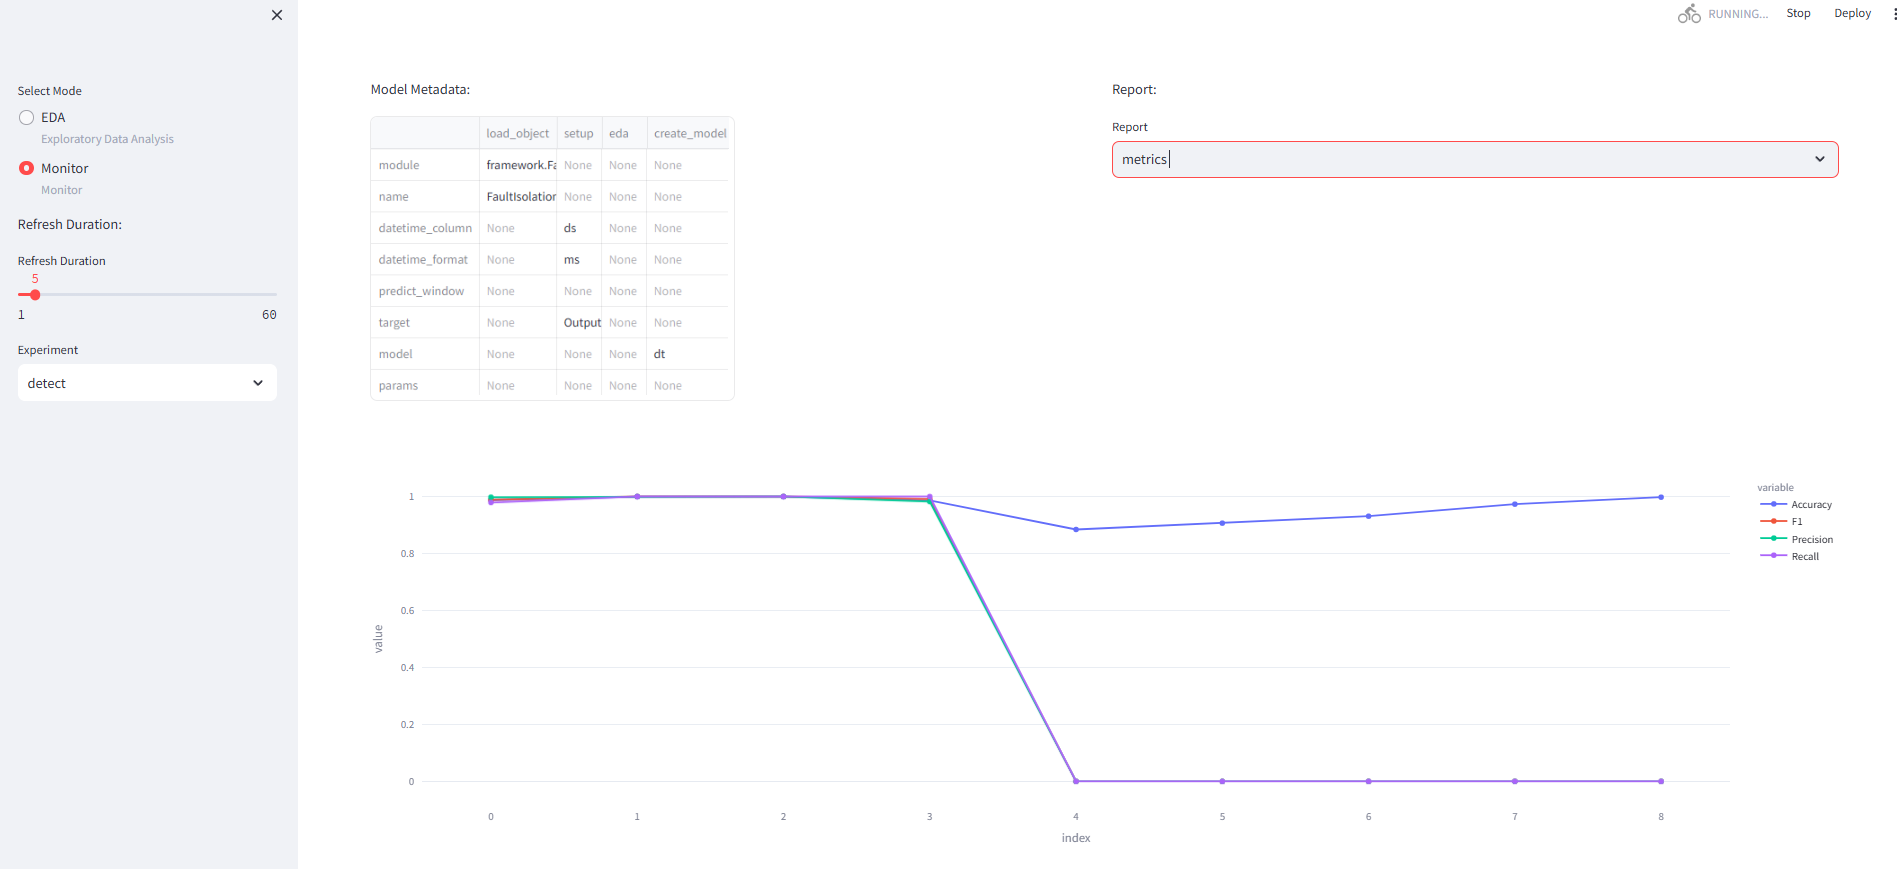
\includegraphics[width=0.9\textwidth, clip, trim={0 0 0 0}]{figs/metrics_filled.png}
% \caption{Model metrics for Electric circuit Decision Tree model after eight prediction calls}
% \label{fi_metrics}
% \end{figure}


\clearpage
\subsection{Fault Detection - PCA} \label{res:fd}


The pump dataset contains 50 sensors, without any labeled one to use fault isolation Experiment on. Therefore, we use the fault detection experiment to find anomalies that could present possible malfunction. In this case, principal component analysis (PCA) is applied with Hotelling's T-squared and SPE/DmodX tests to find the outliers \citep{Taskesen_pca_A_Python_2020}. Listing \ref{lst:pca} presents the configuration file sent to the Experiment Hub service. In this case, we did not enable EDA function, which was done by commenting the keyword out in the configuration file. %\todo[inline]{Ez az utolsó mondat kell?}


\begin{listing}[ht]
\begin{minted}[
    gobble=4,
    frame=single,
    linenos
  ]{yaml}
    ## This is the configuration file FaultDetectionExperiment, 
    ##specifying a PCA instance.
    load_object : ## this is a must
    ##- should not remove - 
    ##unique dynamic import of class 
    ##(dynamic package download is not yet supported)
      module: framework.FaultDetection  
      name: FaultDetectionExperiment
    setup: # from this key, it is arbitrary 
    ##-> the key name is a function 
    ##in the experiment, and the value is the 
    ## parameter of the function.
        # MUST NOT HAVE A 'data' KEYWORD!
        datetime_column : "ds"
        datetime_format : "ms"
    #eda: # Commenting out disables the feature
    create_model :
        model : "pca" #"ee" #"dbscan" #"pca" 
        # If model is none, then compare model is used.
        params:
\end{minted}
\caption{Configuration file for Decision Tree-based fault isolation.}
\label{lst:pca}.
\end{listing}


The PCA model provides a performance figure with showing the variances for the PCs. This is presented on Figure \ref{variance}. The first two PCs account for 60\% of the variance.

\begin{figure}[h!]%
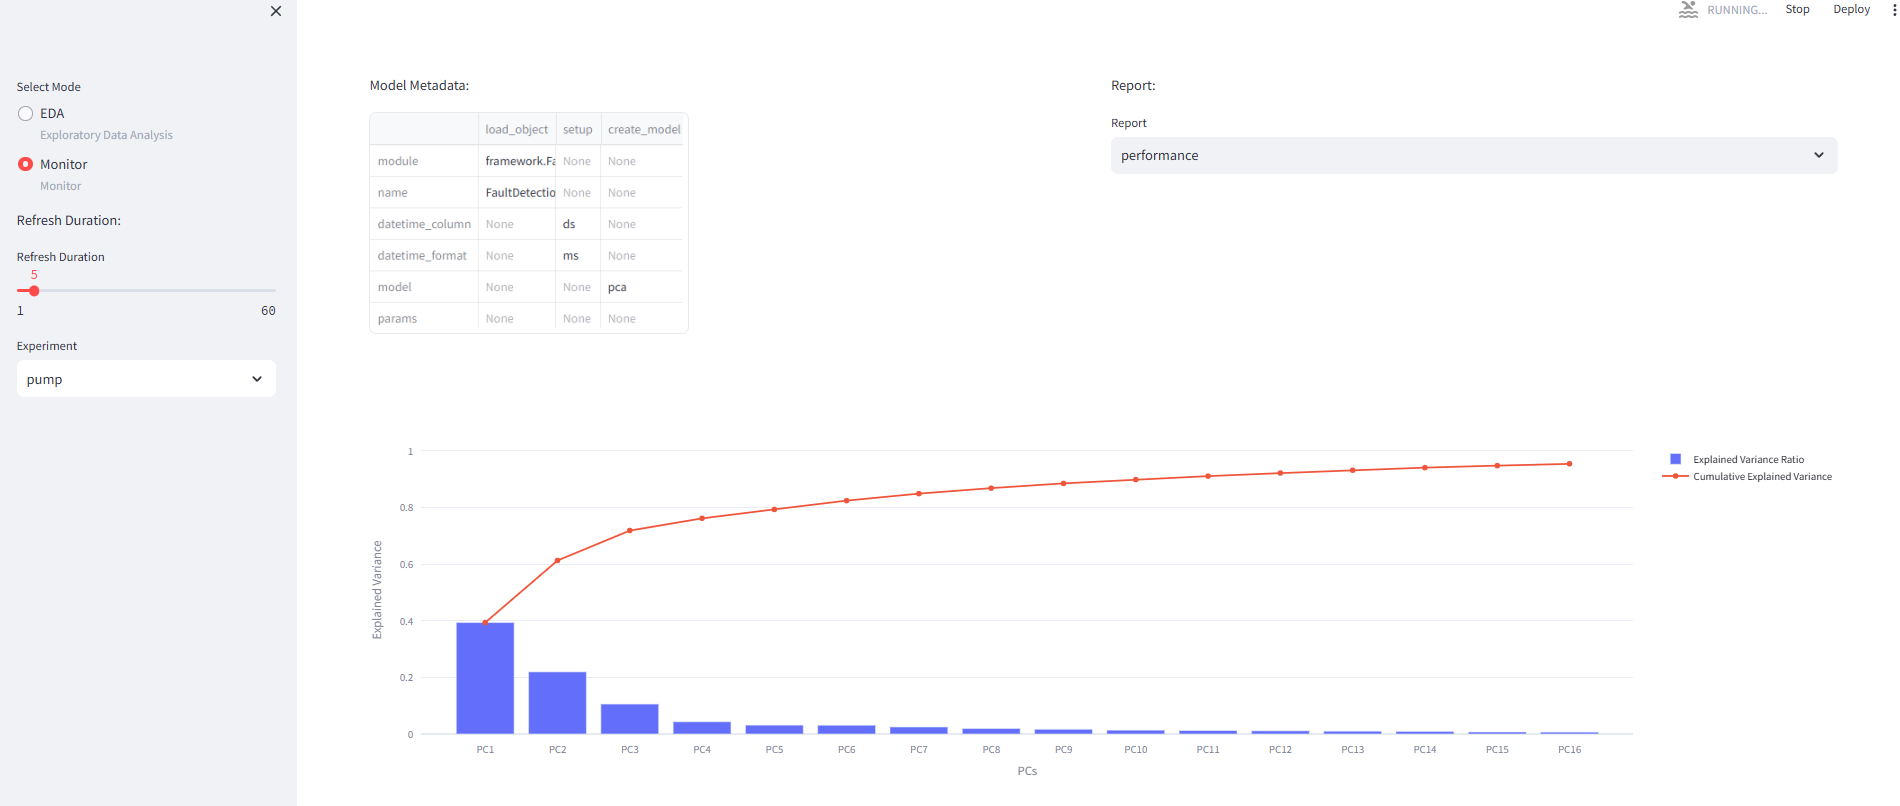
\includegraphics[width=0.9\textwidth, clip, trim={0 0 0 0}]{figs/variancia.png}
{\caption{Variance of the Principal components from the pump dataset}
\label{variance}}
\end{figure}

We also provide a dynamically updating figure called "outliers" to adjust for incoming data. Figure \ref{pca_outliers} presents the anomalies with time on the x-axis, and PC on the y-axis. The blue dots are considered outliers by the Hotelling T-squared tests, the purple shows if a score is an outlier for both tests.

\begin{figure}[h!]%
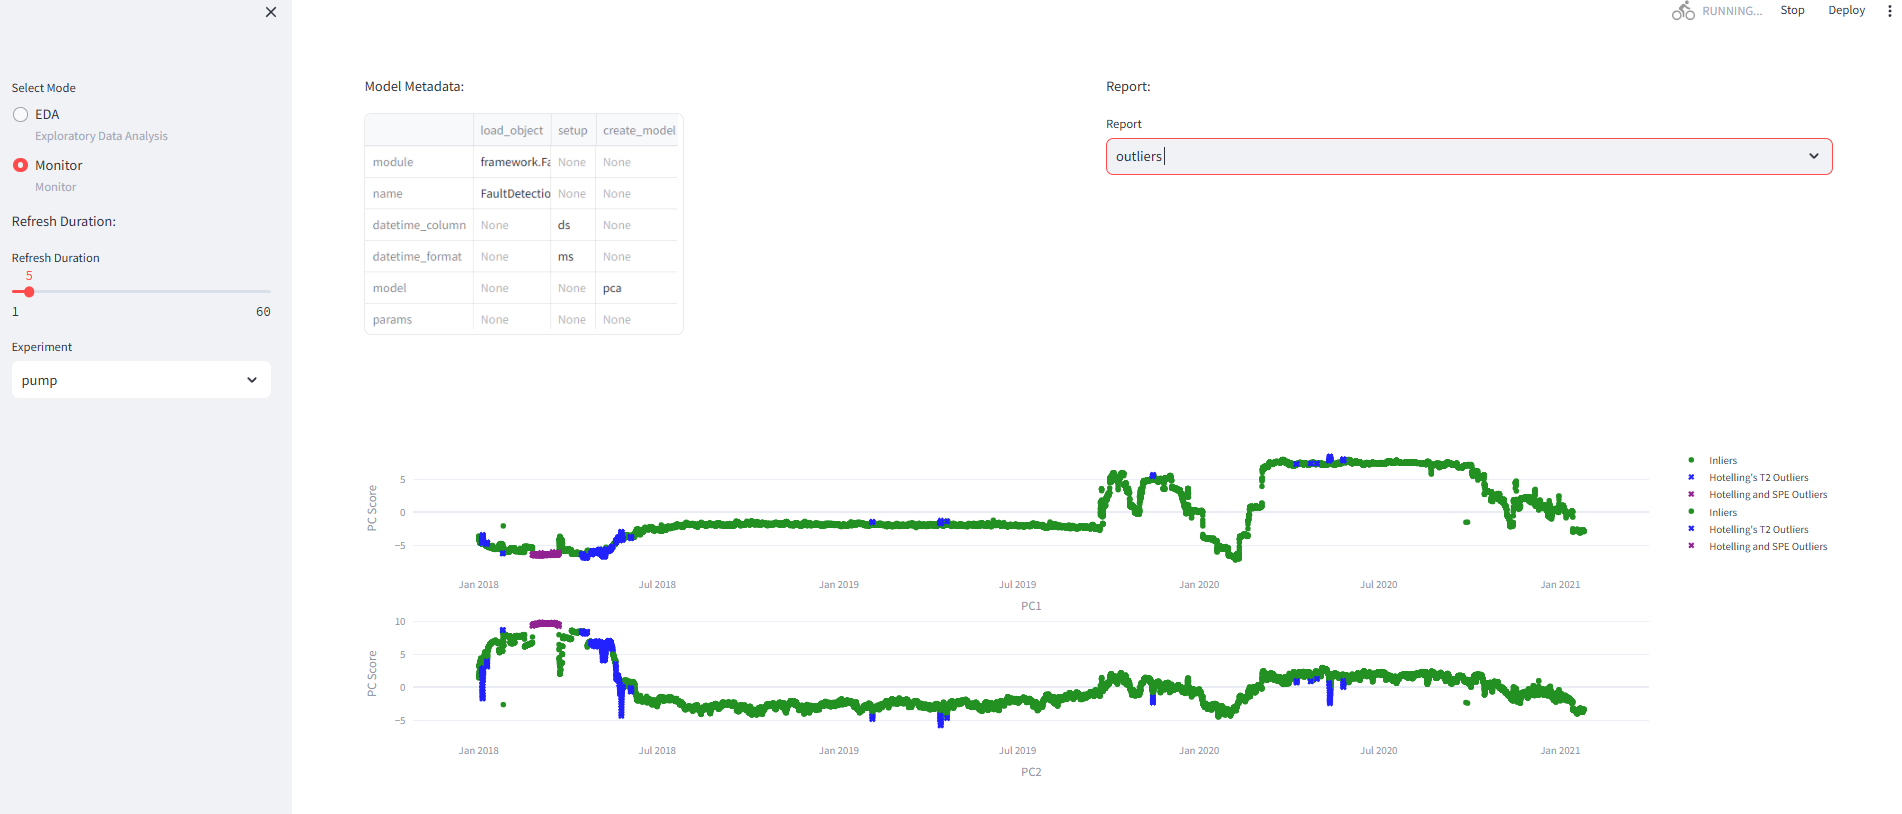
\includegraphics[width=0.9\textwidth, clip, trim={0 0 0 0}]{figs/pca_outliers.png}
{\caption{Outliers in the Principal components from the pump dataset}
\label{pca_outliers}}
\end{figure}




\clearpage

\section{Impact}

The ObServML package opens up new possibilities in the field of real-time monitoring, fault detection, and predictive maintenance in compact and modular industrial environments. Its adherence to MLOps principles, modular microservice-based architecture, and flexible model integration allow it to have a significant impact across research, practice, and industry.

ObServML enables research into adaptive monitoring strategies, data-driven fault isolation without labeled data, and automated retraining mechanisms in environments with limited computational resources. The support for both traditional models (e.g., PCA, ARIMA) and advanced methods (e.g., LSTM, Autoencoders) in a plug-and-play configuration invites comparative studies on model performance across industrial scenarios. Furthermore, its support for experimental process mining methods introduces new possibilities for studying operator behavior and machine log sequences, areas typically under-explored due to a lack of integrative tooling.

The software significantly reduces the overhead for researchers conducting fault detection and isolation (FDI) by automating the model training, deployment, and retraining pipeline within a reproducible framework. Compared to traditional pipelines that require manual scripting and orchestration, ObServML enables faster experimentation and deployment through a unified API and configuration management via Hydra. Prior works like BibMon \cite{MELO2024100182} offer similar analytics capabilities, but lack the deployment-ready MLOps integration that ObServML provides. By decoupling model design from data engineering tasks, the framework streamlines the pursuit of predictive maintenance research as emphasized in Zonta et al. \cite{ZONTA2020106889}.

% ObServML simplifies the workflow of engineers and operators by offering an intuitive Streamlit-based interface, allowing users to monitor anomalies and model outputs without needing programming expertise. It abstracts the complexity of setting up data pipelines, model training, and deployment by encapsulating it in a Docker-based microservice environment. As a result, daily tasks related to monitoring and model management have become significantly more efficient and accessible, especially for non-programmers.

The package was specifically designed with small- and medium-sized industrial enterprises in mind, focusing on real-time process monitoring and predictive maintenance. It is already being tested and developed in industrial settings, ensuring that its functionalities address practical operational needs. Although widespread adoption is still in progress, the software is openly available via GitHub and DockerHub, and early use within academic-industrial collaborations confirms its usability in both research and production environments.


% Impact ->
% ------
% Újratanítás + Performance monitoring
% Belerakni a retraininget

% Funkciók, hogyan valósítja meg az Mlops-OT egyes funkciók

% \textit{This is the main section of the article and reviewers will weight it appropriately.
% Please indicate:}
% \begin{itemize}
%     \item \textit{Any new research questions that can be pursued as a result of your software.}
%     \item \textit{In what way, and to what extent, your software improves the pursuit of existing research questions.}
%     \item \textit{Any ways in which your software has changed the daily practice of its users.}
%     \item \textit{How widespread the use of the software is within and outside the intended user group (downloads, number of users if your software is a service, citable publications, etc.).}
%     \item \textit{How the software is being used in commercial settings and/or how it has led to the creation of spin-off companies.}
%     \end{itemize}
% \textit{Please note that points 1 and 2 are best demonstrated by
%   references to citable publications.}

\section{Conclusions}

This paper presented a Python package designed for compact and modular monitoring applications, addressing key challenges in fault detection and isolation (FDI). By integrating MLOps principles, the framework ensures reproducibility, scalability, and adaptability, making it a versatile solution for industrial environments. Its modular design simplifies the customization of models to suit diverse datasets and operational needs, while its operator-friendly interface streamlines real-time monitoring and deployment processes.

The integration of Docker, RabbitMQ, and MLflow reinforces the application through micro-service architecture, enabling seamless workflow management and efficient communication between components. 


Future work includes expanding model options, enhancing automation features, and integrating advanced visualization tools to further optimize usability. This framework sets a strong foundation for scalable, modular, and user-focused FDI solutions, bridging the gap between technical complexity and operational simplicity in industrial systems.

\section*{Acknowledgements}
This work was supported by the the PIACI-KFI research development program of the National Research, Development and Innovation Office (2020-1.1.2-PIACI-KFI-2020-00062)

The research presented in the article was carried out within the framework of the Széchenyi Plan Plus program with the support of the RRF-2.3.1-21-2022-00008 project.

\bibliographystyle{elsarticle-num} 
\bibliography{cas-refs.bib}

%% else use the following coding to input the bibitems directly in the
%% TeX file.

% \begin{thebibliography}{00}

% %% \bibitem{label}
% %% Text of bibliographic item

% \bibitem{} Use this style of ordering. References in-text should also use a similar style.

% \end{thebibliography}

\textit{If the software repository you used supplied a DOI or another
Persistent IDentifier (PID), please add a reference for your software
here. For more guidance on software citation, please see our guide for
authors or \href{https://f1000research.com/articles/9-1257/v2}{this
  article on the essentials of software citation by FORCE 11}, of
which Elsevier is a member.}

\large{\textbf{Reminder: Before you submit, please delete all 
the instructions in this document, 
including this paragraph. 
Thank you!}}




\end{document}
\endinput
%%
%% End of file `SoftwareX_article_template.tex'.

%%% Local Variables:
%%% mode: latex
%%% TeX-master: t
%%% End:
